\chapter{Ejemplos Sencillos}

%    En este capitulo se van a explicar los conceptos matemáticos utilizados con un ejemplo, para luego aplicarlos al estudio del caso que nos interesa. Se va a calcular la función $\zeta _A (s)$ mediante distintas técnicas, calculando asintóticamente los autovalores, y luego ponerlos en la definición o en el Heat Kernel, y luego se procedió a utilizar el calculo completo
    
    En este capitulo se van a explicar los concepctos matemátocps utilizados con varios ejemplos, para luego poder aplicarlos al operador diferencial que nos interesa, se va a calcular la funcion $ \zeta _A (s) $ de dos maneras distintas y luego se van a calcular sus respectivas energías de vacio.

\section{Dirichlet,Neumann y Periodicas}

En estudiará el espectro del operador diferencial $A = - \partial ^2 _x$, con autovalor $\omega ^2$, al aplicarle distintas condiciones de contorno: \\

\textbf{Dirichlet}

El operador $A$ estrá dado por:

\begin{equation}
\begin{array}{c}
	A \phi (x) = - \partial _x ^2 \phi (x) \\
    \phi (0) = \phi(L) = 0 
\end{array}
\end{equation}



Cuyos autovalores y autofinciones estan dados por  : 

\begin{equation}
\begin{array}{c}
	\phi (x) _n = \sqrt{\frac{2}{L}} Sin( \frac{n \pi x}{L} ) \\
	\omega _n ^2 = \left( \frac{n \pi }{L} \right) ^2 \\
	n = 1,2,3, ...
\end{array}
\end{equation}

La funcion $\zeta _A (s)$ quedará determinada por:

\begin{equation}
\zeta _A (s) = 
\sum _{n=1} ^{\infty} \omega ^{-2s} =  
\left( \frac{\pi}{L} \right) ^{-2s} \sum _{n=1} ^{\infty} n ^{-2s} = 
\left( \frac{\pi}{L} \right) ^{-2s} \zeta (2s)
\end{equation}

Que es regular en $s=-1/2$, entonces la energía de vacío será:

\begin{equation}
E _0 = - \frac{\pi}{12 L}
\end{equation}

Lo cual conduce a una Energía de Vacio atractiva.

\textbf{Neumann}

El operador $A$ estrá dado por:

\begin{equation}
\begin{array}{c}
	A \phi (x) = - \partial _x ^2 \phi (x) \\
    \phi ' (0) = \phi ' (L) = 0 
\end{array}
\end{equation}



Cuyos autovalores y autofinciones estan dados por  : 

\begin{equation}
\begin{array}{c}
	\phi (x) _n = \sqrt{\frac{2}{L}} Cos( \frac{n \pi x}{L} ) \\
	\omega _n ^2 = \left( \frac{n \pi }{L} \right) ^2 \\
	n = 0,1,2,3, ...
\end{array}
\end{equation}

La funcion $\zeta _A (s)$ qserá la misma que la calculada anteriormente, así como tambien la energía de vacio \\

\textbf{Periódicas}

Las condiciones de contorno estan dadas por : 

\begin{equation}
\begin{array}{c}
    \phi (0) = \phi (L)  \\ 
\end{array}
\end{equation}

Cuyos autovalores y autofinciones estan dados por  : 

\begin{equation}
\begin{array}{c}
	\phi _{n=0} = \sqrt{\frac{1}{L}} \\ 
	\phi _{n \neq 0 } (x) = \sqrt{\frac{2}{L}} Cos( \frac{2 n \pi x}{L} ) \\
	\omega _n ^2 = \left( \frac{2 n \pi }{L} \right) ^2 \\
	n = 0,1,2,3, ...
\end{array}
\end{equation}

La funcion $\zeta _A (s)$ queda determinada por:

\begin{equation}
\zeta _A (s) = 
\sum _{n=0} ^{\infty} \omega ^{-2s} =  
\left( \frac{2 \pi}{L} \right) ^{-2s} \sum _{n=1} ^{\infty} n ^{-2s} = 
\left( \frac{2 \pi}{L} \right) ^{-2s} \zeta (2s)
\end{equation}

Que al igual que en los casos anteriores es regular en $s=-1/2$, obteniendo entonces para la Energía de Vacio:

\begin{equation}
E _0 = - \frac{\pi}{6 L}
\end{equation}

Lo cual conduce a una Energía de Vacio atractiva

\section{Condiciones de Contorno Mixtas}

\begin{equation}
\begin{array}{c}
    A \phi (x) = - \partial ^2 _x \ \phi (x)  \\
    \phi (0) = 0 \\ 
    \partial _x \phi (L) + \gamma \phi (L) = 0
\end{array}
\end{equation}

Donde las condiciones de contorno me fijan un espectro autovalores $\omega > 0 $, que está dado cualquiera de las dos ecuaciones equivalentes: 

\begin{equation}
\begin{array}{cc}
    \frac{\omega}{\gamma}  \ Cos( L \omega ) +   Sin( L \omega ) = 0 \\
    \frac{\omega}{\gamma}  + Tg(\omega L )  = 0 
\label{autovalores}
\end{array}
\end{equation}

Una vez obtenidos los autovalores el siguiente paso es calcular la funcion $\zeta$ definida por:

\begin{equation}
    \zeta _ {A } (s) = \sum_{n = 1} ^{ \infty } \omega _n ^ {-2 s}
\end{equation}

Al no poder encontrar explícitamente los autovalores se proceden a distintas técnicas para hallar distintas aproximaciones de la función $\zeta _A (s)$

\subsection{Calculo Asintótico de los autovalores}


Haciendo el cambio a variables adimensionales $\mu = \omega \gamma $ y $\theta = \gamma L $ las ecuaciones (\ref{autovalores}) se pueden expresar de la forma:

\begin{equation}
\begin{array}{c}
    Tg[\mu] + \frac{\mu}{\theta} = 0 \\
    \frac{\mu}{\theta} Cos[\mu] + Sin[\mu] = 0
\end{array}
\label{eq.asintota}
\end{equation}

Tal como se puede ver en la figura [\ref{fig:Dibujo}], los autovalores $\mu _n$ tienden a pegarse a la asíntota vertical de $ Tg [ \mu ] $ a medida que $\mu _n$ se hace cada vez mas grande.

\begin{figure}
    \centering
    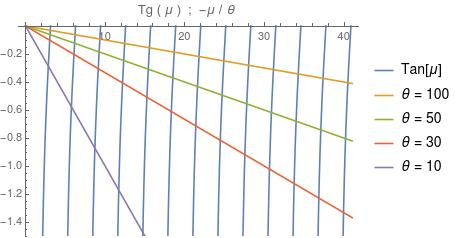
\includegraphics[scale=0.6]{Dibujo.jpg}
    \caption{En este ejemplo, se puede ver que la interseccion entre $Tan[x]$ y $-x$ tiende a las asintotas verticales de la tangente, el mismo comportamiento se aprecia para cualquier $ \theta $.}
    \label{fig:Dibujo}
\end{figure}

Se puede ver entonces de los autovalores $\mu _n$ se pueden descomponer en una parte correspondiente a las asíntotas verticales de $Tg[\mu]$ mas una corrección que tiende a cero a medida que n tiende a $\infty$

\begin{equation}
\begin{array}{c}
    \mu _n = n \pi + \frac{\pi}{2} + \epsilon _n \\
    Donde \ \epsilon _n \rightarrow{0}  \ cuando \ n \rightarrow{0}
\end{array}
\label{eq.mu}
\end{equation}


conocer $\epsilon _n $ es equivalente a resolver la ecuación (\ref{eq.asintota}), la cual no puede resolverse analíticamente, en vez de eso voy a obtener un desarrollo de $\epsilon _n $ para $n \rightarrow \infty$.

voy a intesertar (\ref{eq.mu}) en la segunda ecuacion de (\ref{eq.asintota}) y desarrollar alrededor de $\epsilon \rightarrow{0}$ obteniendo:

\begin{equation}
\begin{array}{c}
    Sin[ n \pi + \frac{\pi}{2} + \epsilon _n ] = 
    - \frac{\mu _n}{\theta}  \ Cos[ n \pi + \frac{\pi}{2} + \epsilon _n ]  \\
 \\

         \sum _{p=0} ^{\infty} \frac{(-1) ^n  \epsilon ^{2 p }}{(2p)!} 
    =  \frac{-1}{\theta}  \ (n \pi + \frac{\pi}{2} + \epsilon ) \
     \sum _{p=0} ^{\infty} \frac{(-1) ^n \epsilon ^{2 p + 1}}{(2p+1)!} 
\end{array}
\end{equation}


Donde acomodando la igualdad, obtengo la ecuacion :

\begin{equation}
    1 = \sum _{p=1} ^{\infty} \epsilon ^{2p+2} \ (-1) ^p
    \left( 
    \frac{1}{(2p+2)!} + \frac{1}{\theta} \frac{(1 )}{(2p+1)!} 
    \right ) +
    \frac{1}{\theta} \left(n \pi + \frac{\pi}{2} \right)
    \sum _{p=0} ^{\infty} \frac{(-1) ^p \epsilon ^{2p+1}}{(2p+1) !}
\label{igualdad epsilon}
\end{equation}

Suponiendo que $\epsilon _n $ tiene un desarrollo en serie de la forma .

\begin{equation}
    \epsilon _n = 
    \frac{\epsilon ^{(1)}}{n}  + 
    \frac{\epsilon ^{(2)}}{n ^2}  + 
    \frac{\epsilon ^{(3)}}{n ^3}  + ...
\label{eq.epsilon}
\end{equation}


Insertando este desarrollo de $\epsilon$ en la ecuación (\ref{igualdad epsilon}), e igualando orden a orden se obtiene, para los primeros ordenes de $\epsilon$:

\begin{equation}
    \epsilon _n = \frac{\theta}{n \pi} 
     - \frac{ \theta}{2 \pi n ^2 } 
\label{epsilons}
\end{equation}

Una vez obtenido el desarrollo de $\mu _n $ puedo calcular $\omega _n = \frac{\mu _n }{L}  $ 



\begin{equation}
    \omega _n = 
	\frac{n \pi}{L} + 
    \frac{\pi}{2 L} +
    \frac{\gamma}{n \pi} +
    \frac{\gamma}{2 n ^2 \pi} +
    O \left(  \frac{1}{n^3} \right) 
\end{equation}
    
Voy a obtener para la funcion $ \zeta _A (s)$ a este orden:
    
\begin{equation}
\begin{array}{cc}
    \zeta _{A} (s) =  \sum _{n=1} ^{\infty} \omega _n ^ {-2 s} =
    \sum _{n=1} ^{\infty} 
    \left(
	\frac{n \pi}{L} + 
    \frac{\pi}{2 L} +
    \frac{\gamma}{n \pi} +
    \frac{\gamma}{2 n ^2 \pi} +
    O \left(  \frac{1}{n^3} \right) 
    \right) ^{-2 s} = \\
    ( \frac{L}{\pi} ) ^{2s}    
    \sum _{n=1} ^{\infty} 
    n ^{- 2 s} 
    \left(
    1 +     
    \underbrace{
        \frac{1}{2 n} + 
        \frac{L \gamma}{n^2 \pi ^2} -
        \frac{L \gamma}{2 n ^3 \pi ^2} +
        O(\frac{1}{n ^{4}} ) } _{ \chi _n}
    \right ) ^{-2 s}
\end{array}
\end{equation}

Para calcular esta serie voy a hacer un desarrollo binomial alrededor de $\chi _n \rightarrow{0} $  .

\begin{equation}
\begin{array}{c}
\zeta _{A} (s) = 
( \frac{L}{\alpha} ) ^{2s}
\sum _{n=1} ^{\infty}
  n  ^{-2 S} \\
(
1 - 2 s \chi _n + 2 s(s+1) \frac{\chi _n ^2}{2} - 2s(2s+1)(2s+2) \frac{ \chi _n ^3}{3!}  + O( \frac{1}{n ^4}) )

\end{array}
\end{equation}

Donde hay que tener en cuenta que cada termino $\chi _{n} ^{m} $ contribuye al orden mas bajo en la sumatoria en una potencia $\frac{1}{n ^m}$, obteniendo como resultado.





\begin{equation}
\begin{array}{c}
    \zeta _A (s) = \left( \frac{L}{\pi} \right) ^{2s} \\
	\Bigg(
		\zeta [2 s] -
		-s \zeta [2s+1 ] +
		 \frac{\zeta [2s +2 ]}{4} \left( 1 - s - s^2 \right) + \\
		 \zeta [2s+3] \left(  
							\frac{s}{12} - \frac{s ^2}{4} - \frac{s ^3}{6} -
							\frac{2 L s \gamma}{\pi ^2} + \frac{2 L s^2 \gamma}{\pi ^2}
		 									\right) 
		+ ...
		\Bigg)
\end{array}
\end{equation}

Se puede ver que el resultado esta expresado como suma de funciones $\zeta (s+n)$ acompañados de unos argumentos $C_{s+n}$ que dependen de losvalores $\alpha,\beta,\gamma, ...$ que estan calculados en la ecuacion (\ref{epsilons}.

Los polos de mi funcion $\zeta _A (s)$ estaran dados por los polos de las funciones $\zeta (s+n)$, desarrollando en los primeros polos obtengo:

\begin{equation}
\begin{array}{c}
\zeta _A (s \rightarrow 1/2) = 
\frac{L}{2 \pi } \frac{1}{s-1/2} + \ finito \\
\zeta _A (s \rightarrow 0) = \ finito \\
\zeta _A (s \rightarrow -1/2) = \frac{\gamma}{2 \pi} \frac{1}{s+1/2} \\
\zeta _A (s \rightarrow -1) = finito \\
\end{array}
\end{equation}

Lo cual corrobora que los polos estan en semienteros de $s$.

\subsection{Calculo de la funcion zeta mediante calculo complejo:}

Conocida la ecuacion de autovalores, se puede proceder a calcular la funcion $\zeta _A (s) $ sin calcular explicitamente los autovalores, utilizando variable compleja.

Donde $\zeta _A (s) $ va a quedar representada por la integral:

\begin{equation}
\begin{array}{c}
   \zeta _A (s) =  \frac{1}{2 \pi i} \int _{C} \frac{f'(x)}{f(x)} z ^{-2s} dz = \\ 
   \\ 
    \frac{1}{2 \pi i} \int _{C}
    \frac{ cos(\gamma z) \left(\gamma + \frac{1}{L} \right) - sin(\gamma z) \frac{z \gamma}{L}
    }
    {cos(\gamma z) \frac{z}{L} + sin(\gamma z)
    }
    z ^{-2 s} dz
\end{array}
\end{equation}

Donde puede utilizarse como camino de integracion cualquiera de los dos caminos representados en la figura [\ref{fig:contorno}], dado que la funcion $f'(z) / f(z) $ tiene polos en los autovalores de $\hat{A}$.






\begin{figure}
\centering
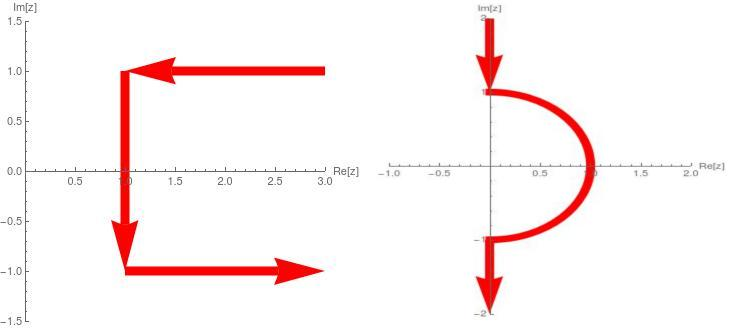
\includegraphics[scale=0.3]{contorno.jpg}
\caption{Camino tenido en cuenta para realizar la integral de contorno en el plano complejo}
\label{fig:contorno}
\end{figure}


Voy a utilizar el camino de la derecha, el cual puedo descomponer en 3 integrales, una angular y dos rectas, la contribución circular es regular para todo s, entonces no aporta a la estructura de polos, en cuanto a las contribuciones del lado recto voy a realizar mi integral en funcion de t, parametrizando z de la forma $z = \pm i L t$ entonces se pueden expresar ambas integrales (luego de tirar los terminos exponencialmente decrecientes)como  :

\begin{equation}
    \frac{Sin(\pi s)}{ \pi } L ^{-2s+1}
    \int _1 ^{\infty} 
    t ^{-2s}
    \underbrace
    {
	\frac{ \frac{1}{L} + \gamma + \gamma t}
	{1+ t}
	} _{\chi}
    dt 
\label{contorno}
\end{equation}

En donde voy a insetar el desarrollo asintotico de   $\chi$. 

\begin{equation}
    \chi = \gamma + \frac{1}{L} \sum _{n=1} ^{\infty} \frac{(-1) ^{n+1}}{t ^n}
\label{eq:chi}
\end{equation}

Luego de integrar termino a termino, obtengo como resultado:

\begin{equation}
    \zeta _A (s) = 
    \frac{Sin(\pi s)}{\pi} L ^{1-2s}
    \left(
    \frac{\gamma}{2s-1} + 
    \frac{1}{L}
    \sum _{n=1} ^{\infty}
    \frac{(-1) ^{n+1}}{2s+n-1}
    \right)
\label{eq.zeta.com}
\end{equation}

De acá se puede ver que tiene polos simples en $s=1/2$ donde la estructura de polos queda determinada por

\begin{equation}
\begin{array}{c}

\zeta(s \rightarrow 1/2) = \frac{\gamma}{2 \pi} \frac{1}{s-1/2} \\
\zeta (s \rightarrow -n - 1/2)  = \frac{ (-1) ^n L ^{2n+1}  }{2 \pi} \frac{1}{s + n + 1/2}

\end{array}
\end{equation}


\subsection{Calculo del Heat-Kernel}

Dado que el operador que estamos autilizando es regular se puede calcular 

\begin{equation}
\begin{array}{c}
\zeta _A (s) = 
\frac{1}{\Gamma (s)} 
\int _0 ^{\infty}
t ^{s-1}
K(t)
dt \\
k(t) = \sum _{n} e^{- \omega _n t}
\end{array}
\end{equation}

Donde se ve que los polos de la funcion $\zeta$ estaran dados por el desarrollo del Heat-Kernel a $t \rightarrow 0 $, el cual admite un desarrollo de la forma

\begin{equation}
K (t) = 
t ^{\frac{-1}{2}}
\sum _{n=0} ^{\infty}
t ^{\frac{k}{2}}
a _k
\end{equation}

Obtengo para los primeros terminos

\begin{equation}
a _0 = 
\frac{1}{\sqrt{4 \pi}}
\int dx =
\frac{L}{\sqrt{4 \pi}} \\
a_1 = 
\end{equation}














